\documentclass[10pt]{beamer}

\usetheme[progressbar=frametitle]{metropolis}
\usepackage{appendixnumberbeamer}

\usepackage[autoplay]{animate}
\usepackage{graphicx}
\usepackage{subcaption}
\usepackage{coloremoji}

\usepackage{booktabs}
\usepackage[scale=2]{ccicons}

%\usepackage{pgfplots}
%\usepgfplotslibrary{dateplot}

\usepackage{xspace}

\newcommand\blfootnote[1]{%
  \begingroup
  \renewcommand\thefootnote{}\footnote{#1}%
  \addtocounter{footnote}{-1}%
  \endgroup
}

\setbeamercolor{normal text}{bg=white}
\newcommand{\themename}{\textbf{\textsc{metropolis}}\xspace}

\title{Första KEGen}
\subtitle{Tmux - \underline{\textbf{T}}erminal \underline{\textbf{mu}}ltiple\underline{\textbf{x}}or}
\date{\today}
\author{Simon Rydell}
\institute{Systecon}

% \titlegraphic{\hfill\includegraphics[height=1.5cm]{logo.pdf}}

\begin{document}

\begin{frame}
\titlepage
\end{frame}

%\maketitle
% 
\begin{frame}{Hello World in tmux}
    \begin{columns}[c]
        \column{2in}
            Shell scripting is a 1950's Jukebox \\
                \ - Larry Wall, \\
                \small grundare av programmeringsspråket perl
        \column{2in}
            \begin{figure}[h!]
                \centering
                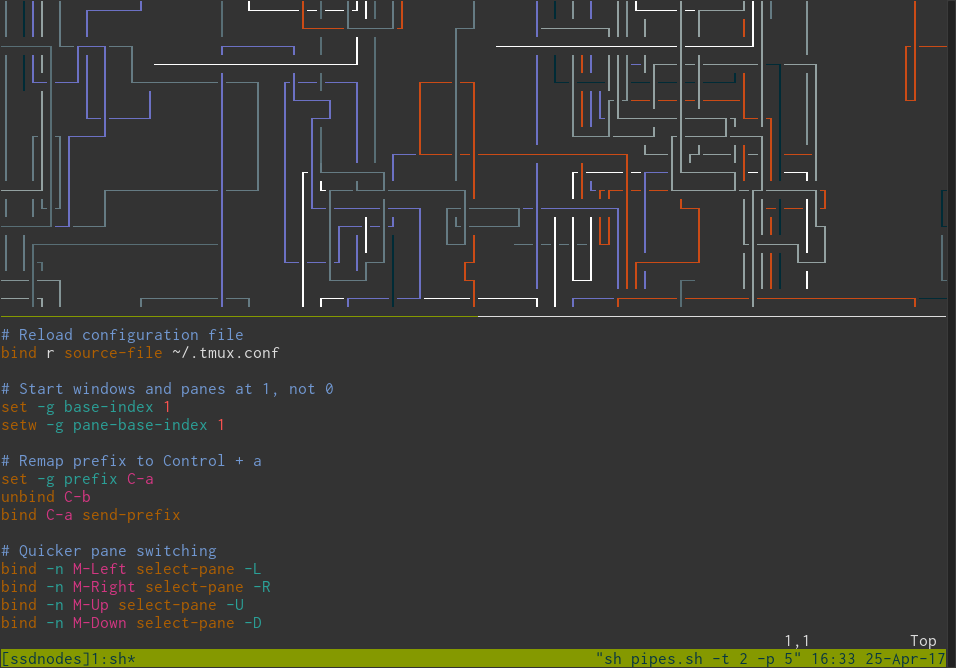
\includegraphics[width=1\textwidth]{../figures/tmux0.png}
            \end{figure}
    \end{columns}
    \blfootnote{github.com/srydell/tmux-intro}
\end{frame}

% 
\begin{frame}{Översikt}
    \setbeamertemplate{section in toc}[sections numbered]
    \tableofcontents[hideallsubsections]
    \blfootnote{github.com/srydell/tmux-intro}
\end{frame}

% --- Section ---
\section{Vad kan man göra från en terminal och varför behöver jag $n$ av dom?}

\begin{frame}{Vad kan man göra från en terminal och varför behöver jag $n$ av dom?}
% First row
    \begin{columns}[c]
        \column{2in}
            Allt som du kan göra "för hand'' med en dator, fast snabbare!
        \column{2in}
            Din tid är viktigare än datorns, så vänta inte på den. Starta en ny terminal!
    \end{columns}
    \blfootnote{github.com/srydell/tmux-intro}
\end{frame}

% --- Section ---
\section{Panes, windows \& sessions}

\begin{frame}{Panes}
    \begin{columns}[c]
        \column{4in}
            \begin{figure}[h!]
                \centering
                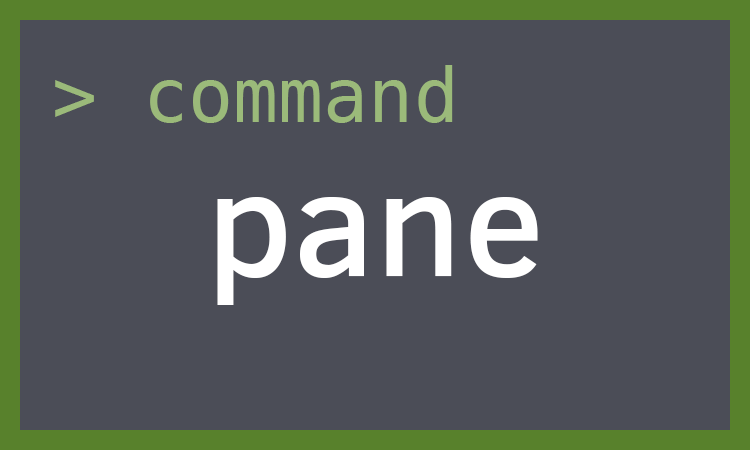
\includegraphics[width=1\textwidth]{../figures/pane.png}
            \end{figure}
    \end{columns}
    \blfootnote{github.com/srydell/tmux-intro}
\end{frame}

\begin{frame}{Windows}
    \begin{columns}[c]
        \column{4in}
            \begin{figure}[h!]
                \centering
                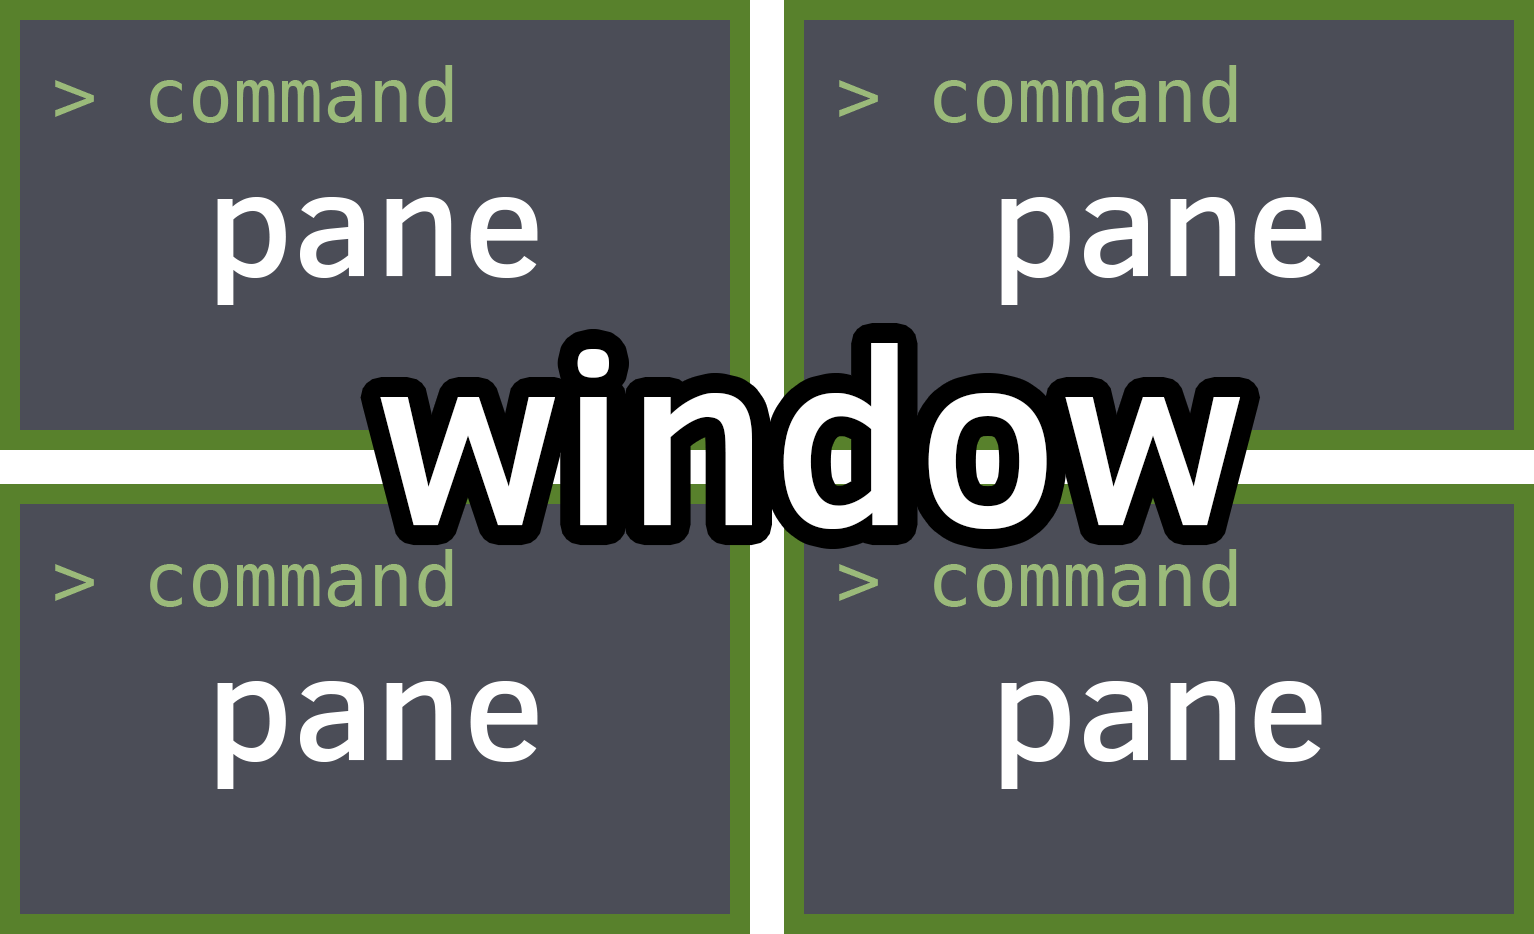
\includegraphics[width=1\textwidth]{../figures/window.png}
            \end{figure}
    \end{columns}
    \blfootnote{github.com/srydell/tmux-intro}
\end{frame}

\begin{frame}{Sessions}
    \begin{columns}[c]
        \column{4in}
            \begin{figure}[h!]
                \centering
                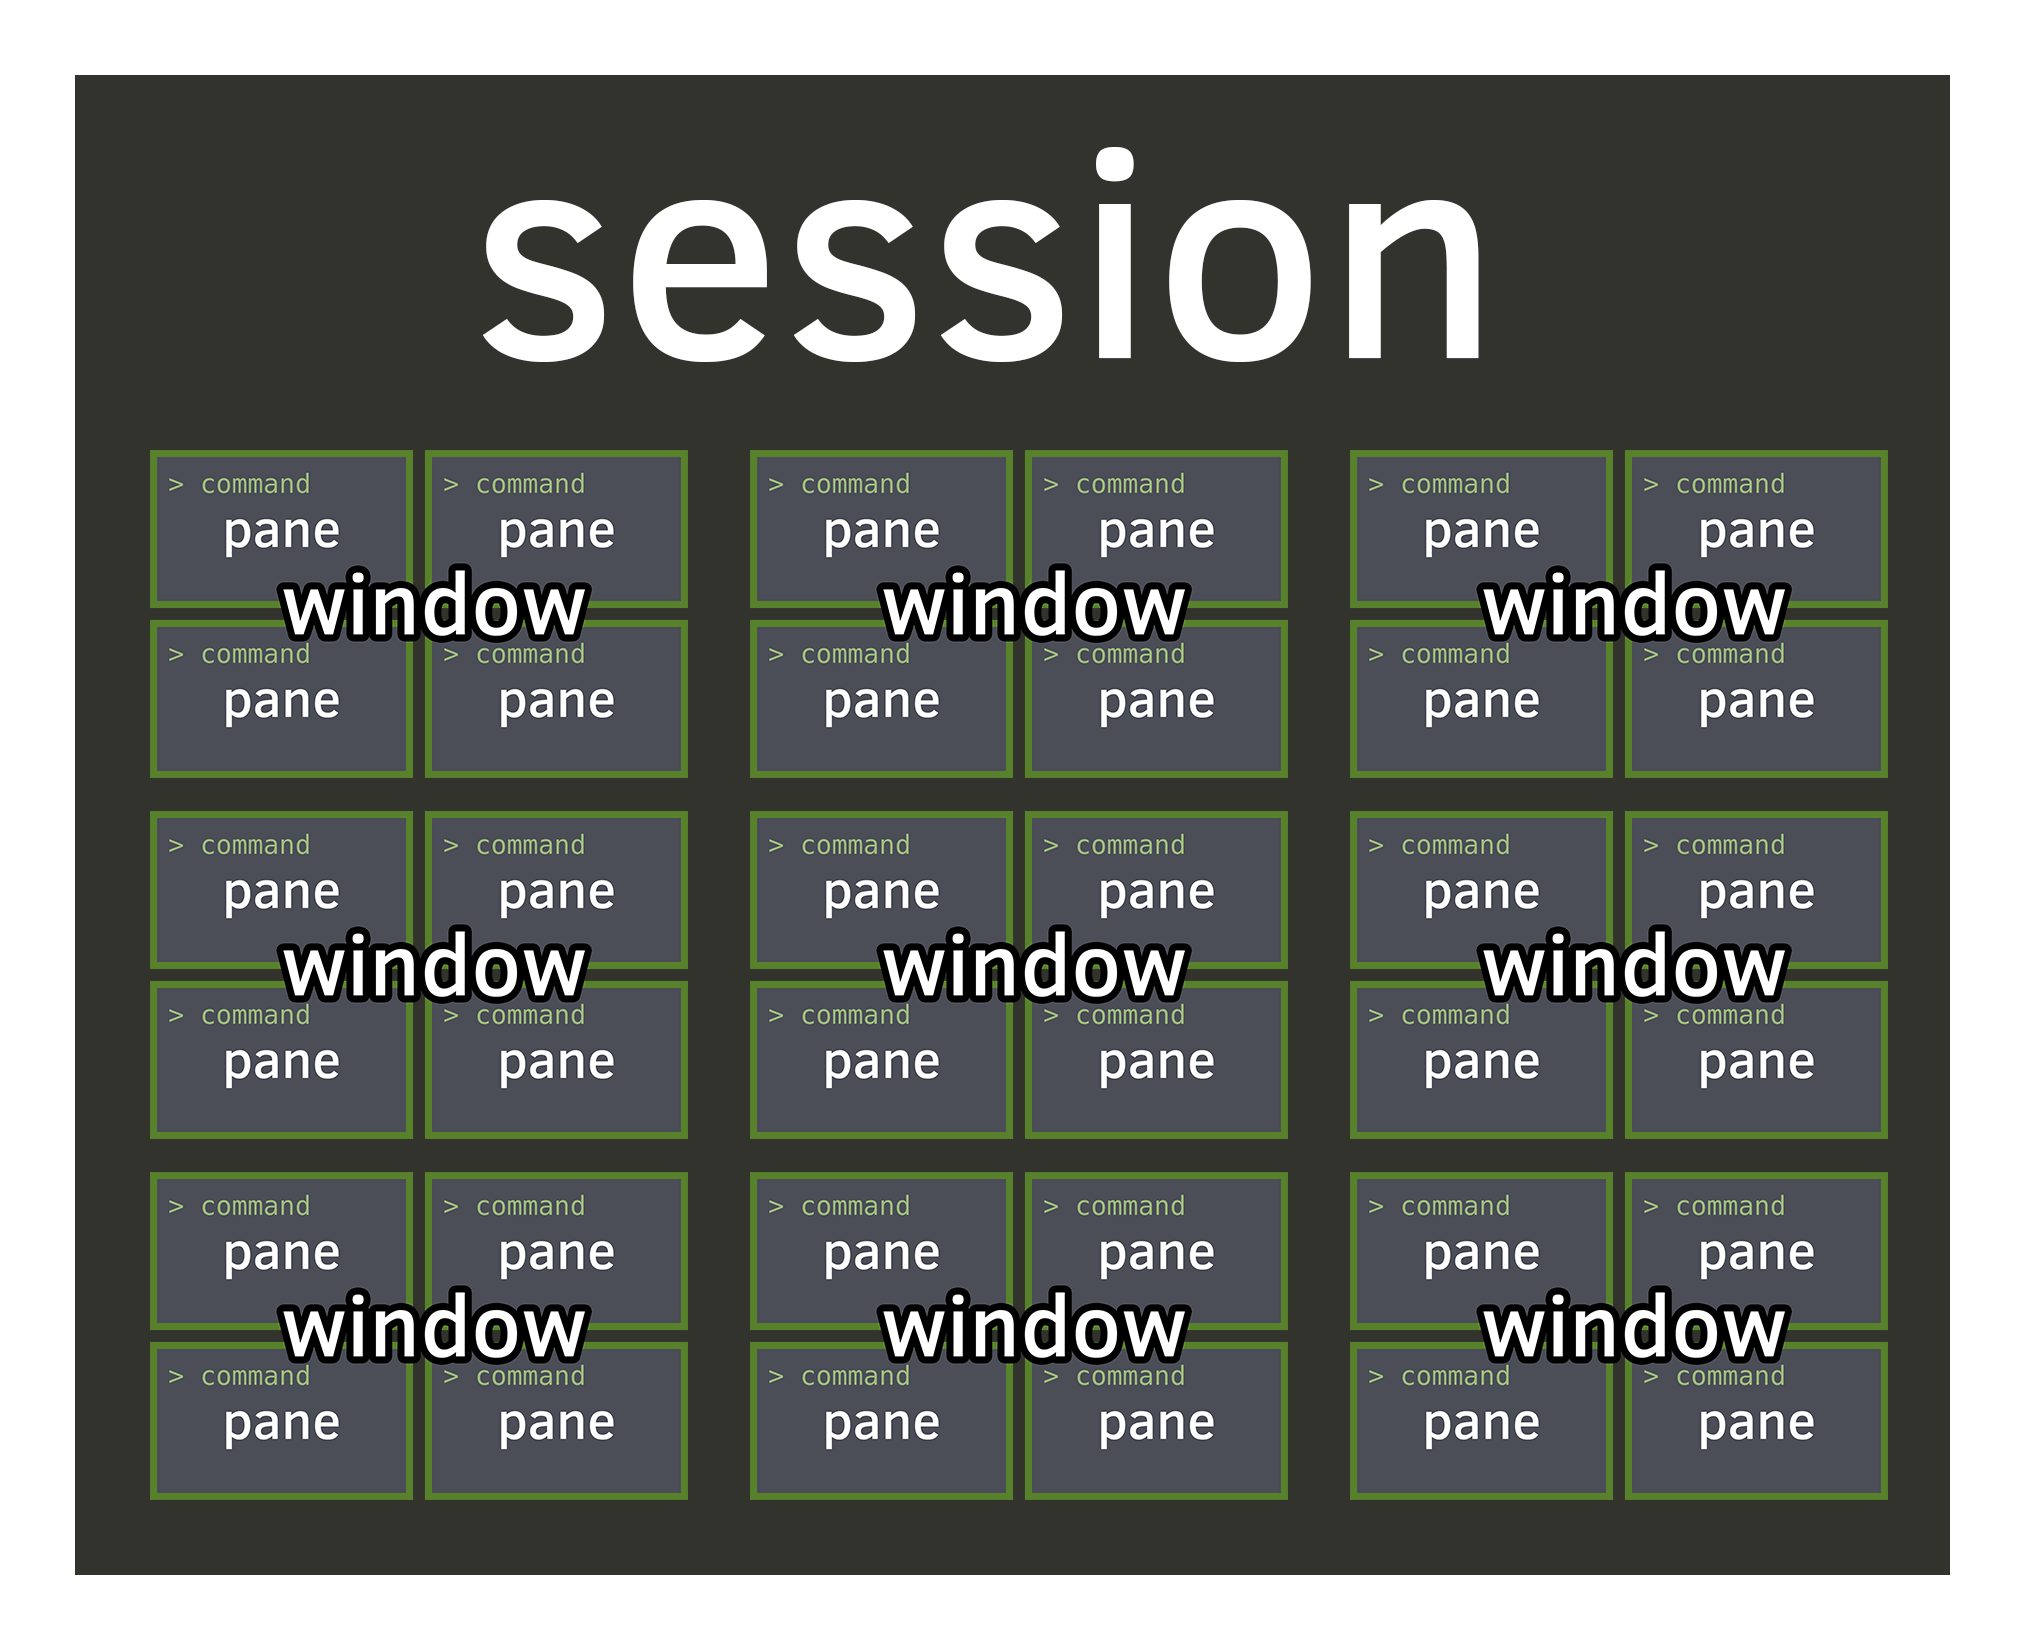
\includegraphics[width=1\textwidth]{../figures/session.png}
            \end{figure}
    \end{columns}
    \blfootnote{github.com/srydell/tmux-intro}
\end{frame}

% --- Section ---
\section{Demo med exempel}

\begin{frame}{Demo}
     \begin{itemize}
         \item Röra sig i tmux (panes, windows \& sessions)
         \item $🐍 + (👶 🐟)$
         \item Dokumentation med Markdown
         \item C++ \& Javascript med Emscripten
     \end{itemize}
     \blfootnote{github.com/srydell/tmux-intro}
\end{frame}

\begin{frame}{Tmux - Terminal multiplexor}
     \begin{center}
         \large Tack!
     \end{center}
     \blfootnote{github.com/srydell/tmux-intro}
\end{frame}


\end{document}